\section{Benchmark Design}
\label{sec:benchmark-design}

\subsection{Source cohorts, frozen models, and representations}

PTB-XL supplies 21,799 twelve-lead ECGs and 49 waveform-derived measurement and morphology concepts~\cite{wagner2020ptbxl}. We use the existing patient-disjoint split: 15,149 records for training, 3,325 for validation, and 3,325 for test. The test set contains 2,862 unique patients. Every model receives the same ordered record manifest, and preprocessing statistics are estimated on training records only. PTB-XL is the source cohort for the primary benchmark. For external validation, we repeat the complete 450-cell multiscale SAE audit on a credentialed, patient-partitioned MIMIC-IV-ECG manifest of 100,000 ECGs from 48,491 patients (Appendix~\ref{app:mimic-replication}).

All six pretrained encoders remain frozen throughout the benchmark. We update no FM parameters and perform no task-specific fine-tuning; only the SAEs are trained on activations extracted from the fixed checkpoints. Each encoder is called through its released preprocessing path (Appendix~\ref{app:model-interfaces}, Table~\ref{tab:multiscale-models}). We audit pre-projection transformer-layer states for CARDIAC-FM; its released 768-to-512 pooled projection is used only in the downstream stage and is not the dimension of the source layer atlas. Consequently, all six source layer atlases have $d=768$.

\begin{figure*}[!t]
  \centering
  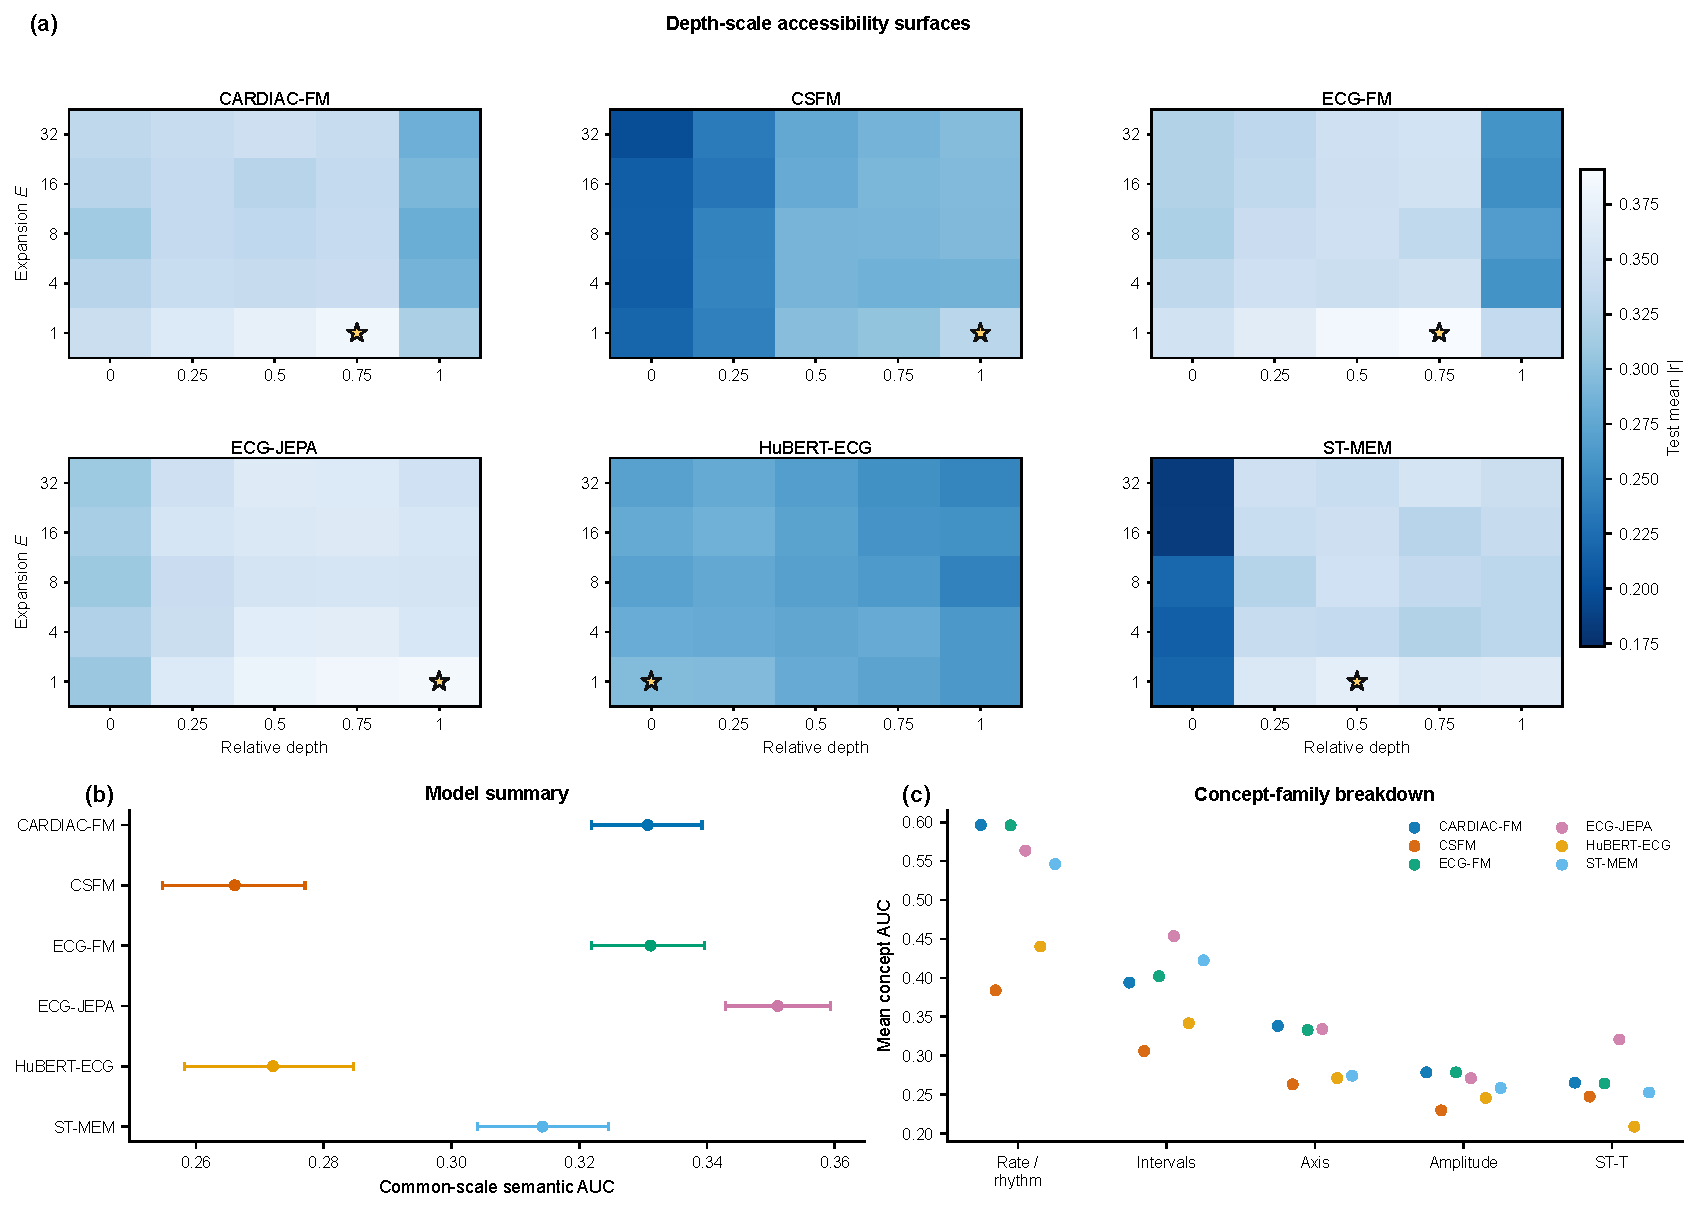
\includegraphics[width=\textwidth]{figures/multiscale_semantic_atlas.pdf}
  \caption{Single-coordinate clinical accessibility across the matched SAE atlas. (a) Test mean absolute concept correlation over five relative depths and five exactly matched expansion factors; circles mark each model's peak cell. (b) Common-scale semantic AUC with paired patient-cluster 95\% intervals. (c) Mean concept-level common-scale AUC by ECG concept family. Features are selected on the training subset and frozen before held-out evaluation.}
  \Description{A three-panel figure shows six depth-scale heatmaps for ECG foundation models, a forest plot of common-scale semantic AUC with confidence intervals, and a dot plot of mean concept accessibility by ECG concept family.}
  \label{fig:semantic-atlas}
\end{figure*}

\begin{figure*}[!t]
  \centering
  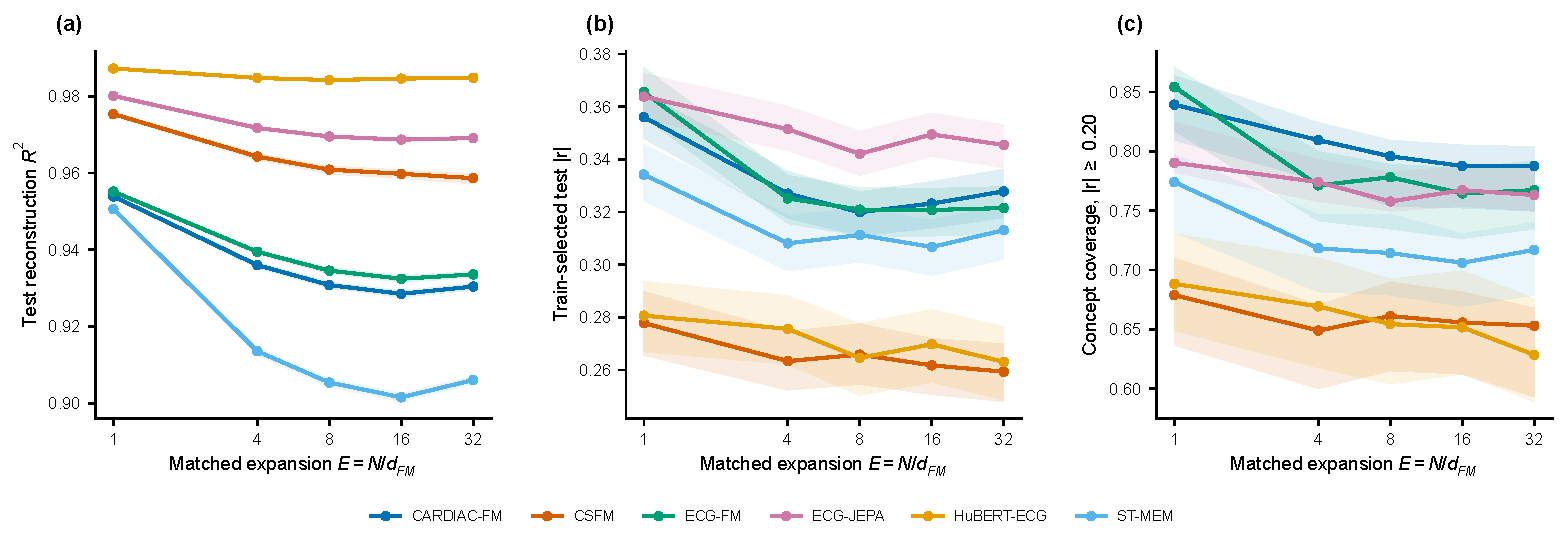
\includegraphics[width=\textwidth]{figures/multiscale_patient_matched_scale_curves.pdf}
  \caption{Patient-bootstrap FM profiles at each common SAE scale: (a) reconstruction $R^2$, (b) train-selected single-coordinate clinical accessibility, and (c) concept coverage at $|r|\geq0.20$. Lines compare models at identical $E$ and therefore identical absolute $N$; bands are paired 95\% patient-cluster intervals.}
  \Description{Three line panels show reconstruction, train-selected single-coordinate clinical accessibility, and concept coverage for six models over five matched expansion factors, with confidence bands.}
  \label{fig:matched-curves}
\end{figure*}

\subsection{Standardized depth and exact scale matching}

For an encoder exposing $L$ audited states, target relative depth $q\in\{0,.25,.5,.75,1\}$ maps to
\begin{equation}
  \ell(q)=\left\lfloor q(L-1)+\tfrac{1}{2}\right\rfloor.
\end{equation}
We record both $q$ and the realized depth $\ell/(L-1)$. CSFM maps to layers $(0,1,3,4,5)$; each 12-state encoder maps to $(0,3,6,8,11)$. Relative depth provides a shared coordinate for aligning early, intermediate, and final representation stages across encoders with different layer counts. This alignment enables systematic depth-wise comparison of where reconstruction fidelity, clinical accessibility, and reproducible sparse structure emerge across models.

For a batch of standardized activations $X\in\mathbb{R}^{B\times d}$, BatchTopK computes positive pre-activations and retains the largest $Bk$ values over the complete batch:
\begin{align}
  P &= \operatorname{ReLU}\!\left((X-b_d)W_e^{\top}+b_e\right),\\
  Z &= \operatorname{BatchTopK}_{Bk}(P), \qquad \widehat{X}=ZW_d^{\top}+b_d.
\end{align}
Decoder columns are constrained to unit norm. Thus $k$ specifies the batch-average active-feature budget, while the reported realized mean $L_0$ summarizes per-record activation sparsity.

The primary grid fixes expansion $E=N/d\in\{1,4,8,16,32\}$ and $k/d=1/8$. Because $d=768$ for every source layer, all models use exactly the same widths
\begin{equation}
  N\in\{768,3072,6144,12288,24576\}
\end{equation}
and the same $k=96$ at every scale. Each SAE is trained for 8,000 steps with batch size 256, Adam learning rate $3\times10^{-4}$, and seed 4311, 4312, or 4313. The complete grid contains
\begin{equation}
  6\ \text{models}\times5\ \text{depths}\times5\ \text{scales}\times3\ \text{seeds}=450
\end{equation}
cells, arranged as 75 blocks in which all six FMs share the same target depth, $N$, $k$, and seed. Primary contrasts pair all models at the same prespecified $E$ and summarize performance over the shared scale grid, with scale choices fixed before test evaluation.

\subsection{Leakage-controlled single-coordinate clinical accessibility}

Concept values are aligned by ECG identifier and standardized with training-split means and standard deviations. A missing or non-finite value is replaced by the training mean, which is zero in standardized coordinates. Coordinate selection uses the same deterministic 4,096-record subset of the training split in every cell. For concept $c$ and SAE code coordinate $j$, let $r^{\mathrm{train}}_{jc}$ denote their correlation on that subset. We select
\begin{equation}
  j_c^*=\arg\max_j |r^{\mathrm{train}}_{jc}|
\end{equation}
once and evaluate the same coordinate on validation and test records. The test single-coordinate accessibility score is the mean $|r^{\mathrm{test}}_{j_c^*c}|$ over 49 concepts; coverage is the fraction with $|r^{\mathrm{test}}_{j_c^*c}|\geq .20$. Training-only selection fixes every SAE coordinate, layer, and scale before held-out evaluation. This estimand quantifies how strongly one sparse coordinate locally exposes each concept, and the $.20$ cutoff provides a consistent descriptive operating point across models.

\subsection{Fixed-scale accessibility calibration}

At the common $E=8$ cells ($N=6144,k=96$), we compare seven readouts: fixed-$\alpha=10$ ridge from the dense state, full SAE code, or 16/four train-ranked SAE coordinates; and fit-free train-selected native, SAE, or random coordinates. Dense coordinates are evaluated once per model--depth, whereas SAE metrics average three seeds. The random control averages 20 shared seeds, each projecting the normalized state onto $N$ Gaussian unit directions before the same ReLU, BatchTopK, batch order, and training-only selection. We report held-out mean $|r|$, coverage at $|r|\geq.20$, paired differences, and random-seed percentile intervals. Coordinates and readout settings are fixed from the training data before validation and test outcomes are used for held-out evaluation.

\subsection{Metric-specific FM profiles}

\paragraph{Measurement fidelity.}
We report normalized reconstruction $R^2=1-\mathrm{SSE}/\mathrm{SST}$, dead-feature fraction, realized mean $L_0$, and the fraction of layer--scale cells satisfying the preregistered validation fidelity gate ($R^2\geq.90$ and dead fraction $<.20$). Reconstruction quantifies how faithfully the sparse instrument preserves a representation and is interpreted alongside clinical accessibility.

\paragraph{Single-coordinate clinical accessibility.}
Train-selected test correlation and concept coverage quantify how locally the fixed concept panel is exposed by individual sparse-code coordinates. Their primary role is relative model comparison under an identical selection and capacity protocol. Joint interpretation with reconstruction fidelity connects local concept exposure to the quality of the underlying sparse decomposition.

\paragraph{Reproducibility.}
Within each model, depth, and scale, we retain up to the 256 most active non-dead decoder directions per seed according to validation firing rate. Hungarian matching maximizes signed decoder cosine for each seed pair. We report matched cosine above a 100-permutation random-pairing floor and normalized overlap between the selected decoder subspaces.

\paragraph{Common-scale summary.}
For metric curve $m(E)$, the model profile is the normalized log-scale area
\begin{equation}
  \operatorname{AUC}_{E}(m)=
  \frac{1}{\log 32-\log 1}\int_{\log 1}^{\log 32}m(e^u)\,du,
\end{equation}
Here, $E$ is the SAE expansion factor, evaluated at $\{1,4,8,16,32\}$, and $m(E)$ may denote reconstruction $R^2$, single-coordinate mean $|r|$, concept coverage, matched decoder cosine, or selected-subspace overlap. We approximate the integral by trapezoidal integration over these five points in $\log E$. Division by $\log 32-\log 1$ makes $\operatorname{AUC}_{E}$ a normalized average across SAE scales. The resulting scale summary is then averaged over the five depths and three seeds as specified by each inferential analysis. Fidelity, single-coordinate accessibility, coverage, and stability jointly define the model's multiscale interpretability profile.

\subsection{Paired uncertainty and multiplicity}

The primary test inference resamples PTB-XL patients with replacement 2,000 times and retains all records belonging to a sampled patient. The sorted patient set and bootstrap seed are identical across all 450 cells, enabling paired FM differences. BatchTopK codes are computed once in the frozen original test order with batch size 256; bootstrap weights are then applied to patient-aggregated sufficient statistics, preserving a common encoding across all resamples. Reconstruction uses the frozen full-test reference mean in the SST term for every bootstrap draw. These intervals quantify held-out patient sampling uncertainty conditional on the frozen reference, FM and SAE weights, and train-selected coordinates. The three SAE seeds are averaged within each draw.

A second 10,000-sample crossed bootstrap resamples the five depth units and three SAE seeds to quantify design variation after integrating the frozen scale curve. Pairwise model contrasts are adjusted by Benjamini--Hochberg within each metric family~\cite{benjamini1995fdr}. Scale sensitivity is summarized by Kendall rank correlation between every pair of common $E$ values. Together, patient and design intervals characterize complementary sources of uncertainty: held-out patient sampling and depth--seed design variation.

\subsection{Sparsity sensitivity}

The primary fixed-$k/d$ arm holds the absolute active budget constant while dictionary width grows. A preregistered mid-depth sensitivity arm instead fixes $k/N=1/64$, giving $k\in\{12,48,96,192,384\}$ over the same five exact widths, six models, and three seeds. At relative depth $q=0.5$, this arm retains the primary training protocol and uses $N=\{768,3072,6144,12288,24576\}$ with $k=N/64=\{12,48,96,192,384\}$. It evaluates the stability of metric-specific FM ordering under an alternative sparsity parameterization, with both arms and their comparison preregistered before test evaluation.

\begin{table*}[t]
  \centering
  \caption{Final-layer input-harmonization audit. $\Delta$ values are changes in test mean $|r|$ from the native protocol. Coverage is the joint-protocol fraction of 49 concepts reaching $|r|\geq0.20$; CKA compares joint and native test representations.}
  \label{tab:input-harmonization}
  \begin{tabular}{lrrrrrr}
    \toprule
    Model & Native mean $|r|$ & $\Delta$ Lead & $\Delta$ Temporal & $\Delta$ Joint & Joint coverage & Joint CKA \\
    \midrule
    CARDIAC-FM & 0.2922 & $+0.0000$ & $-0.0058$ & $-0.0058$ & 0.857 & 0.991 \\
    CSFM       & 0.3321 & $-0.0004$ & $+0.0000$ & $-0.0004$ & 0.837 & \textbf{1.000} \\
    ECG-FM     & 0.3166 & $-0.0000$ & $-0.0048$ & $-0.0048$ & \textbf{0.959} & 0.997 \\
    ECG-JEPA   & \textbf{0.4380} & $+0.0000$ & $+0.0000$ & $+0.0000$ & \textbf{0.959} & \textbf{1.000} \\
    HuBERT-ECG & 0.2923 & $\boldsymbol{+0.0006}$ & $\boldsymbol{+0.0005}$ & $\boldsymbol{+0.0006}$ & 0.735 & \textbf{1.000} \\
    ST-MEM     & 0.3891 & $-0.0000$ & $-0.0131$ & $-0.0131$ & 0.898 & 0.770 \\
    \bottomrule
  \end{tabular}
\end{table*}

\begin{table*}[t]
  \centering
  \small
  \caption{MIMIC-IV-ECG held-out multiscale SAE profiles. Reconstruction, semantic alignment, and coverage are normalized expansion-curve AUCs averaged over five relative depths. Stability is matched decoder-feature cosine across SAE seeds; subspace stability is normalized overlap of the selected decoder subspaces. Higher is better except for dead-feature fraction.}
  \label{tab:mimic-model-profiles}
  \begin{tabular}{lrrrrrr}
    \toprule
    Model & Recon. & Semantic & Coverage & Dead fraction & Feature stability & Subspace stability \\
    \midrule
    CARDIAC-FM & 0.958 & 0.295 & 0.674 & 0.166 & 0.366 & 0.718 \\
    CSFM       & 0.979 & 0.261 & 0.582 & 0.380 & 0.293 & \textbf{0.778} \\
    ECG-FM     & 0.955 & 0.282 & 0.625 & \textbf{0.099} & \textbf{0.378} & 0.702 \\
    ECG-JEPA   & 0.985 & \textbf{0.324} & \textbf{0.781} & 0.447 & 0.340 & 0.748 \\
    HuBERT-ECG & \textbf{0.990} & 0.279 & 0.610 & 0.546 & 0.323 & 0.762 \\
    ST-MEM     & 0.960 & 0.274 & 0.600 & 0.211 & 0.348 & 0.760 \\
    \bottomrule
  \end{tabular}
\end{table*}
